\documentclass{article}

\usepackage{geometry}
\usepackage{inconsolata}
\usepackage[T1]{fontenc}

% font setup from Cody Cutler's thesis
\usepackage{amssymb}
%\usepackage[defaultsans]{lato}
%\usepackage[lf,footnotefigures]{MinionPro} % After amssymb
\usepackage[toc,bib]{tabfigures}

% No Minion Pro?  Uncomment the next line to use Times
%\usepackage{times,mathptmx}
%\usepackage{crimson}
\usepackage[bitstream-charter]{mathdesign}
\usepackage{mathrsfs}

% adapted from https://github.com/jonhoo/thesis/

% for 1.5 line spacing
\usepackage{setspace}
\onehalfspacing

% set up nicer headers/footers (in particular, no capitalization and put page
% number in footer)
\makeatletter
\def\ps@headings{\let\@mkboth\markboth
    \def\@oddfoot{\hfil \rm\thepage \hfil}
    \def\@evenfoot{\hfil \rm\thepage \hfil}
    \def\@evenhead{\hfil \sl \leftmark}	% Left heading.
    \def\@oddhead{\hbox{}\sl \rightmark \hfil}	% Right heading.
    \def\chaptermark##1{\markboth {\ifnum \c@secnumdepth >\m@ne
	\@chapapp\ \thechapter. \ \fi ##1}{}}
    \def\sectionmark##1{\markright {\ifnum \c@secnumdepth >\z@
	\thesection. \ \fi ##1}}
    \pulldownheader				% Bring header down from edge
}
\makeatother

%\pagestyle{headings}

% more colors (like RedOrange)
\usepackage[dvipsnames]{xcolor}

% qualitative colors
% subset of https://jfly.uni-koeln.de/color/
% that is also distinctive in grayscale
\definecolor{set1}{HTML}{0071b2} % blue
\definecolor{set2}{HTML}{e59c00} % orange
\definecolor{set3}{HTML}{009e73} % green
\definecolor{set4}{HTML}{efe440} % yellow

% so we can splice in PDFs
\usepackage{pdfpages}

% set up bibliography
\usepackage[square,comma,numbers,sort&compress]{natbib}

% enumerate* and itemize*
\usepackage[inline]{enumitem}

% for \begin{comment}
\usepackage{verbatim}

% for source-code listings
% (latex.out fixes compatibility with latexrun, see
% https://github.com/aclements/latexrun/issues/13#issuecomment-322550767)
\usepackage[newfloat,outputdir=latex.out]{minted}
\setminted[rust]{frame=lines}
\setminted[c]{frame=lines}

% for formulas
\usepackage{mathtools}

% to split lists into multiple columns
\usepackage{multicol}

% for "on page NN" reference
\usepackage[nospace]{varioref}

% for \ifoptionfinal
\usepackage{ifdraft}

% for nice tables
\usepackage{booktabs}
\usepackage{multirow}
\usepackage{array,ragged2e}

% \xspace
\usepackage{xspace}

% subfigures
\usepackage{subcaption}
% default space between figure and caption
\captionsetup[figure]{skip=0.5\baselineskip}

% fpeval (to add numbers)
\usepackage{xfp}

\usepackage[breaklinks, pdfborder={0 0 0}]{hyperref}
\usepackage[nameinlink]{cleveref}

\hypersetup{
    colorlinks=true,
    linkcolor=set1,
    filecolor=magenta,
    urlcolor=set1,
    citecolor=set3,
    pdftitle={Verifying a concurrent file system with sequential reasoning},
    pdfauthor={Tej Chajed},
}

% set the format of figure numbers
\renewcommand{\thefigure}{\arabic{chapter}-\arabic{figure}}
\newcommand{\eg}{{e.g.},\xspace}
\newcommand{\ie}{{i.e.},\xspace}

% restore these definitions to color wp/wpc and braces
% \newcommand{\syntax}[1]{\textcolor{blue}{#1}}
% \newcommand{\syntaxbraced}[1]{\cleft[blue]\{#1\cright[blue]\}}
\newcommand{\syntax}[1]{#1}
\newcommand{\syntaxbraced}[1]{\{#1\}}

\usepackage{pftools}
\usepackage{amsmath}
\usepackage{amssymb}

% used in \loc macro
\usepackage{numprint}

% some sanity for special characters
\usepackage[utf8]{inputenc}
\input{glyphtounicode}
\pdfgentounicode=1

% generate synctex output for inverse search
\synctex=1

% gnuplot figures have some page group issue, see
% https://tex.stackexchange.com/questions/76273/multiple-pdfs-with-page-group-included-in-a-single-page-warning
\pdfsuppresswarningpagegroup=1

%% do not reset page numbers at \mainmatter
%\let\mainmatterorig\mainmatter
%\renewcommand\mainmatter
% {\edef\p{\arabic{page}}%
%  \mainmatterorig
%  % we need to compute the actual current page number. we know the page number
%  % from _before_ we called \mainmatter. but what is it now? well, it is
%  % certainly that +1. but we also need to account for the next chapter starting
%  % on a "right" (odd) page. we do this by adding the page number modulo two.
%  % TODO: double check before final version
%  \setcounter{page}{\p+1+(\p-\p/2*2)}%
% }

% adding TODOs
\newcommand{\insertnote}[3]{\noindent\textcolor{#1}{\textbf{#2:} #3}}
\newcommand{\note}[1]{\insertnote{blue}{NOTE}{#1}}
\newcommand{\todocite}[1]{\textcolor{red}{[cite #1]}}

% https://tex.stackexchange.com/questions/52697/automated-lists-for-todos-in-latex-document
\newcounter{todo}
\newcommand\todo[1]{\refstepcounter{todo}\textcolor{red}{#1}%
\addcontentsline{tod}{subsection}{\thetodo.~(\S\thesection)~#1}}%
\makeatletter
\newcommand\listoftodos{%
  \pdfbookmark{todo list}{Contents}
  \chapter*{List of TODOs}\@starttoc{tod}}
\makeatother

% out of habit this macro is called \lyt, even though all TODOs are written by
% and assigned to me
\newcommand{\lyt}[1]{\textcolor{red}{\textbf{LYT:}} \todo{#1}}

% a command to indicate current editing progress
\newcommand{\resume}{
  \begin{center}
    \color{set2}
    \hrule \vspace{1pt} \hrule \hrule
    \vspace{10pt}
    \textbf{This section is not yet complete.}
    \vspace{10pt}
    \hrule \hrule \vspace{1pt} \hrule
  \end{center}
}

\usepackage{relsize}
% sets monospace font
\renewcommand{\ttdefault}{pxtt}


% must be last in usepackage list!
\usepackage{hyperref}
\usepackage{cleveref}

% other stuff
\newcommand{\mydate}{February 14, 2023}
\newcommand{\mycompletion}{May 25, 2024}
\newcommand{\mytitle}{Helping Web Developers Give Users Control Over Their Data}
\newcommand{\mytimeline}{\vspace{1em}\noindent\textbf{Timeline} }

\author{
    Lillian Tsai\\
    Massachusetts Institute of Technology\\
    \texttt{tsilyai@mit.edu}
}

\date{\mydate}

\title{\mytitle}

\begin{document}

% -*- TeX-master: "paper.tex"; TeX-PDF-mode: t -*-

\title{Thesis Proposal: Helping Web Developers Give Users Control Over Their Data}
\author{Lillian Tsai}
\prevdegrees{
  A.B., Harvard University (2017) \\
  S.M., Harvard University (2017)}
\department{Department of Electrical Engineering and Computer Science}
\degree{Doctor of Philosophy}
\degreemonth{May}
\degreeyear{2024}
\thesisdate{May 13, 2024}
\supervisor{M. Frans Kaashoek}{Charles Piper Professor of Electrical Engineering and Computer Science}
\cosupervisor{Malte Schwarzkopf}{Professor of Computer Science, Brown University}
\chairman{Leslie A. Kolodziejski}{Professor of Electrical Engineering and
  Computer Science \\ Chair, Department Committee
  on Graduate Students}


\newpage

\maketitle

\section{Introduction}%
%\label{ch:introduction}
Users' privacy requirements for their sensitive data on web applications are
highly contextual and constantly in flux. For example, a user might wish to hide
and protect data of an e-commerce or dating app profile when inactive, but also
want their data to be present should they return to use the application. 
%
%But today, achieving this flexible privacy remains out of reach, in part
%because of the many challenges facing web developers in building services that
%can adapt to changing privacy needs. 
Today, however, services often provide only coarse-grained, blunt tools that
result in all-or-nothing exposure of users' private information, and fail to
achieve the flexible privacy that users want and deserve.
%

%
This thesis introduces the notion of \emph{disguised data} for flexible data
privacy. Disguised data is a reversible state of data in which sensitive data is
selectively hidden.
%
To demonstrate the feasibility of disguised data, this thesis also presents
\sys---the first system for disguised data---which helps web applications allow users
to remove their data without permanently losing their accounts, anonymize their
old data, and selectively dissociate personal data from public profiles.
%
\sys lets developers support these features while maintaining application
functionality and referential integrity via \emph{disguising} and \emph{revealing}
transformations.
%
Disguising selectively renders user data inaccessible via encryption, and
revealing enables the user to restore their data to the application.
%
%\sys's techniques allow transformations to compose in any order, \eg deleting a
%previously anonymized user's account, or restoring an account back to an
%anonymized state.
%

%
In this chapter, we motivate the need for data disguising for flexible
privacy; describe the challenges in successfully disguising and revealing data;
and introduce our approach to achieve data disguising as well as our
contributions.

%*********************************************************************************%
%*********************************************************************************%
%*********************************************************************************%
\section{Motivation} 
Many users today have tens to hundreds of accounts with web services that store
sensitive data, from social media to tax preparation and e-commerce
sites~\cite{tens,hundreds,password_life_cycle}.
%
And while users now have the right to delete their data (via \eg the
GDPR~\cite{eu:gdpr} or CCPA~\cite{ccpa}), users want and deserve more nuanced
controls over their data that don't exist today.
%

Consider Twitter: after a change in management~\cite{musk-twitter}, many users
wanted to leave the platform and try out alternatives (\eg
Mastodon~\cite{mastadon}).  But each user faced a tricky question: should they
keep their Twitter account, or should they delete it?
%
Advice on how to quit Twitter~\cite{quit-twitter-india, quit-twitter-mash}
highlight how keeping an inactive account leaves sensitive information (\eg
private messages) vulnerable on Twitter's servers; but deleting the account
prevents the user from changing their mind and coming back, causing them to
permanently lose all their followers and content.  Hence, many users left
Twitter but kept their accounts~\cite{nbc-twitter,shondarhimes,kenolin}.
%
A better solution would let users temporarily revoke Twitter's access to their
data while having the option to come back.

Similarly, users give dating apps personal data, and frequently deactivate and
reactivate their accounts.
%
This sensitive data should be protected from the application and potential data
breaches~\cite{tinder, okcupid} when a user deactivates their account, but be
readily available when they choose to return.

Users may also prefer old data, such as past purchases in an online store or
their passport details with a hotel, to be inaccessible to the service after
some time of inactivity, and therefore protected from leaks or service
compromises~\cite{retention,breach:marriott}. Or users may prefer
to---explicitly or automatically---dissociate their identity from old data, such
as teenage social media posts or old reviews on HotCRP.
%
Today, users work around the lack of such support by explicitly maintaining
multiple identities (\eg Reddit throwaway accounts~\cite{reddit:throwaway} and
Instagram ``finstas''~\cite{nytimes:finsta}), an inflexible and laborious
solution.
%

%
Providing this functionality can benefit both the service and the user.
%
It helps the service comply with privacy regulations, reduces its liability on
data breaches, and appeals to privacy-conscious users; meanwhile, the user can
rest assured that their privacy is protected, but can also get their data back
and reveal their association with it if they want.


%*********************************************************************************%
%*********************************************************************************%
%*********************************************************************************%
\section{Disguised Data: A New Abstraction for Flexible Privacy}
%
This desired flexible privacy functionality describes an in-between state of
user data in web applications: where users are not quite gone, because they can
return to the application; but they are also not quite there, because some or
all of their data has been removed.
%

%
To capture this new state of data, this thesis introduces the new key
abstraction of \emph{disguised data}.  Disguised data represents a state of data
where \one{} some or all of the user's original sensitive data is rendered
inaccessible to the application; \two{} some data may be replaced with
placeholders to keep the application structure intact (\eg placeholder parent
comments to maintain comment thread structure); and \three{} the data can be
restored with the user's authorization.
%

%
Systems for disguised data move closer to an Internet where
users can leave services and return at any time, where old data on servers is
protected by default, and where services provide users with control over their
identifying data visible to the service and other users.
%

%*********************************************************************************%
%*********************************************************************************%
%*********************************************************************************%
\section{Challenges} 
Today, disguised data for flexible privacy remains out of reach for users of
web applications in part because getting it right is hard. 
%
Real applications have complex notions of privacy, data ownership, and data
sharing.
%
Simple solutions that \eg delete all data associated with a user can break
referential integrity or create orphaned data, which requires application
changes to handle correctly, and lack support for users to return.
%
To solve this manually, a developer would have to carefully perform
application-specific database changes to remove data, store any data removed to
be able to later restore it, and correctly revert the database changes on
restoring.

%
Developers would also have to reason about interactions between multiple
data-redacting features, and how these features would compose.
%
For example, imagine an application that supports both account deletion and
anonymizing old data: if a user wants to delete all their posts after they have
been anonymized, a SQL query must somehow determine which anonymized posts
belong to the user in order to remove them.
%
And if the user later wants to return, the developer must account for the
applied anonymization and restore posts as anonymized.
%

%
Furthermore, stored removed data must be inaccessible to the application and
protected against data breaches, but must be accessible if the user chooses to
return. The developer also needs to provide user-friendly ways for users to
prove their ownership of the stored data.
%


%*********************************************************************************%
%*********************************************************************************%
%*********************************************************************************%
\section{Our Approach}
%
To realize disguised data, we present a general system that helps developers
specify and apply two kinds of transformations: \emph{\xxing transformations},
which move the user's data into a disguised state; and \emph{revealing
transformations}, which restore the original data at a user’s request.
%
\Xxing transformations aim to protect the confidentiality of users' \xxed data
(\eg links to throwaway accounts or old HotCRP reviews) even if the application
is later compromised (\eg via a SQL injection or a compromised admin's account).
%

%
We demonstrate our approach in \sys, a system that realizes disguising and
revealing transformations for database-backed web applications via a set of
primitives that have well-defined semantics and compose cleanly.
%
Developers specify the transformations that their application should provide,
and \sys takes care of correctly applying, composing, and optionally reverting
them, while maintaining application functionality and referential integrity.
%

%
%\section{Challenges}
%
Our approach for \sys's approach faces three challenges, and we describe each
challenge and our solution's abstractions next.

\subsection{Disguise Specifications}
%
First, \sys needs to present a simple, yet versatile interface for developers to
specify \xxing transformations.
%
\sys addresses this challenge with a restricted programming model centered
around three primitives: remove, modify, and decorrelate (which reassigns data
to placeholder users).
%
This model limits the potential for developer error, and lets \sys derive the
correct \xxing and revealing operations, while supporting a wide range of
transformations.
%

%
\subsection{Pseudoprincipals}
Second, to work with existing applications in practice, \sys's \xxing
transformations should require minimal application modifications.
%
To achieve this, \sys introduces \emph{pseudoprincipals}, anonymous placeholder
users that are inserted into the database on \xxing and exist solely to own data
decorrelated from real users (\eg because the application requires the data to
continue operating) and maintain referential integrity.
%
Pseudoprincipals can also act as built-in ``throwaway accounts,'' as they let
the user disown data after-the-fact, as well as potentially later reassociate
with it.
%
To correctly reason about ownership when data may be decorrelated multiple times
(\eg by global anonymization after throwaways have been created), \sys maintains
an encrypted \emph{speaks-for chain} of pseudoprincipals that only the original user
can unlock and modify.
%

%
\subsection{Diff Records and Reveal Credentials}
Third, \sys needs to have access to the original data for users to be able to
reveal their data and return to the application, but the whole point is to make
that data inaccessible to the service.
%
While \sys could ask users to store their own \xxed data, this would be
burdensome.
%
Instead, \sys stores the \xxed data on the server in encrypted form as
\emph{diff records}, and unlocks
and restores data to the service only when a user provides their \emph{reveal
credentials} (\eg a password or a private key).

%
\section{Contributions}
%
The main contribution of this thesis is the identification and exploration of
\emph{disguised data} for flexible user data privacy in web applications. As
part of this, this thesis contributes:

\begin{enumerate}[nosep]
    \item The abstraction of \emph{data disguising via \xxing and revealing
        transformations}, including 
        %abstractions for developers and users of web applications, 
        %including \xxing and revealing transformations;
        disguise specifications written with a small, composable set of
        data-anonymizing primitives (remove, modify, and decorrelate to
        pseudoprincipals), and reveal credentials to allow users
        to reveal their data (Ch.~\ref{ch:overview}).
        %, which cover a wide range of application
        %needs and compose cleanly; 

    \item Design techniques to realize disguised data, including diff records and speaks-for chains.
        (Ch.~\ref{ch:design})

    \item \sys, a prototype Rust library for MySQL-backed web applications that
        implements user data control via disguising and revealing, which is
        open-source at
        \url{https://github.com/tslilyai/edna} (Ch.~\ref{ch:impl}).

    \item Case studies that integrate \sys with three real-world web
    applications and demonstrate \sys's ability to enable composable and
        reversible transformations. (Ch.~\ref{ch:case_studies})

    \item An evaluation of \sys's effectiveness and performance, including how
    \sys contrasts with and complements related work (Qapla~\cite{qapla} and
        CryptDB~\cite{cryptdb}) (Ch.~\ref{ch:eval}) 
\end{enumerate}
%

%\subsection{Limitations}
%
While disguised data can help developers to add more flexible user data
controls, the abstraction and its implementation in \sys have some limitations. 
%
First, disguised data is a concept scoped for single applications, and does not
tackle the problem of data sharing between services.
%
%While \sys enables \xxing and revealing transformations in a broad class of
%applications, \sys has some limitations.
%
\sys also assumes bug-free \xx specifications, and that applications use \sys
correctly.
%
Furthermore, \sys does not aim to protect un\xxed data in the database against compromise;
combining \sys with an encrypted database can add this protection.
%
Finally, attacks to identify users from \sys's metadata (\eg the size of
stored \xxed data) or placeholder data left in the database (\eg embedded text)
are out of scope.
%



\iffalse
\section{Remaining Work: Revealing with Schema Migrations and Application
Updates}

In \sys's current design, \textbf{application updates} that implicitly enforce
invariants on application data remain unknown (and thus uncheckable) by \sys.
\sys also fails to reveal disguised data affected by \textbf{schema migrations}
performed since the time of disguise.
%
We will add an API for developers to log important updates and schema migrations with \sys, which \sys will apply to disguised data prior to restoring it to the database.

\sys will apply these updates or schema migrations prior to performing \sys's
existing consistency checks; these checks enable \sys to detect if revealing
transformations will violate referential integrity or other structual database
invariants (\eg uniqueness requirements). 

\fi


\section{Background and Related Work}%
%\label{ch:related}
\subsection{Encrypted Data Storage}
CryptDB, Mylar

\subsection{Policy-Enforcing Systems}
Qapla


\section{Approach}%
%\label{ch:research}
%
To tackle the problem of flexible privacy in web applications, we present a
system design that moves closer to an internet where users can leave services
and return at any time, where old data on servers is protected by default, and
where services provide users with control over their identifying data visible to
the service and other users.

%
Our approach is to create a general system that helps developers specify and
apply two kinds of transformations: \emph{\xxing transformations}, which render
all or some of the user’s original sensitive data inaccessible to the
application; and \emph{revealing transformations}, which restore the original
data at a user’s request.
%
\Xxing transformations aim to protect the confidentiality of users' \xxed data
(\eg links to throwaway accounts or old HotCRP reviews) even if the application
is later compromised (\eg via a SQL injection or a compromised admin's account).
%

%
We demonstrate our approach in \sys, a system that realizes disguising and
revealing transformations for database-backed web applications via a set of
primitives that have well-defined semantics and compose cleanly.
%
Developers specify the transformations that their application should provide,
and \sys takes care of correctly applying, composing, and optionally reverting
them, while maintaining application functionality and referential integrity.
%

%
\subsection{Challenges}
%
We had to address three challenges to make this approach work.
%
First, \sys needs to present a simple, yet versatile interface for developers to
specify \xxing transformations.
%
\sys addresses this challenge with a restricted programming model centered
around three primitives: remove, modify, and decorrelate (which reassigns data
to placeholder users).
%
This model limits the potential for developer error, and lets \sys derive the
correct \xxing and revealing operations, while supporting a wide range of
transformations.
%

%
Second, to work with existing applications in practice, \sys's \xxing
transformations should require minimal application modifications.
%
To achieve this, \sys introduces \emph{pseudoprincipals}, anonymous placeholder
users that are inserted into the database on \xxing and exist solely to own data
decorrelated from real users (\eg because the application requires the data to
continue operating) and maintain referential integrity.
%
Pseudoprincipals can also act as built-in ``throwaway accounts,'' as they let
the user disown data after-the-fact, as well as potentially later reassociate
with it.
%
To correctly reason about ownership when data may be decorrelated multiple times
(\eg by global anonymization after throwaways have been created), \sys maintains
an encrypted speaks-for chain of pseudoprincipals that only the original user
can unlock and modify.
%

%
Third, \sys needs to have access to the original data for users to be able to
reveal their data and return to the application, but the whole point is to make
that data inaccessible to the service.
%
While \sys could ask users to store their own \xxed data, this would be
burdensome.
%
Instead, \sys stores the \xxed data on the server in encrypted form, and unlocks
and restores data to the service only when a user provides their credentials to
reveal.
%

\subsection{\sys Overview}

\begin{figure}[t!]
  \centering
    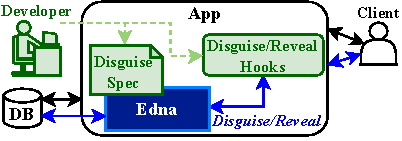
\includegraphics{figs/edna_overview}
    \caption{Developers write \xx specifications and add hooks to invoke \sys
        from the application (green); in normal operation, clients use these
        hooks in the application to \xx and reveal their data in the database
        (blue).
    }
  \label{f:edna-overview}
\end{figure}

\begin{figure}[h]
  \centering
  \begin{subfigure}[h]{0.5\columnwidth}
  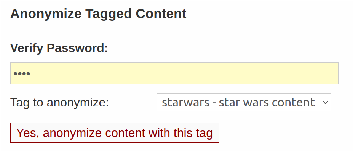
\includegraphics[width=\columnwidth]{figs/lobsters_catanon}
  \end{subfigure}
  \begin{subfigure}[h]{\columnwidth}
  \begin{lstlisting}[language=Ruby,escapeinside={(*}{*)}]
  def tag_anon
    # instantiate the disguise spec with the provided tag to anonymize
    disg_spec = edna.instantiate_spec("tag_anon.json",params[:tag])
    # apply the disguising transformation
    disg_id = edna.apply_disguise(@user.id,params[:passwd],disg_spec)
    # email the disguise ID to the user to allow revealing
    SendDisguiseEmail(@user, disg_id)
  end
  \end{lstlisting}
  \end{subfigure}
  \vspace*{-1em}
  \caption{The Lobsters developer adds a hook in the UI and code to perform
      topic-based anonymization.}
  \label{f:lobsters_hook}
  \end{figure}

%
\sys helps developers realize new options for users to control their data
via \emph{\xxing transformations}.
%
The developer integrates an application with \sys by writing \xx specifications
and adding hooks to \xx or reveal data using \sys's API
(Figure~\ref{f:edna-overview}).
%
This proceeds as follows:
%

%
(1) An application registers users with a public--private keypair
that either the application or the user's client generates; \sys stores the
public key in its database, while the user retains the private key for use in
future reveal operations.
%

%
(2) When the application wants to \xx some data, it invokes \sys with the
corresponding developer-provided \xx specification and any necessary
parameters (such as a user ID).
%
\Xx specifications can remove data, modify data (replacing some or all of its
contents with placeholder values), or decorrelate data, replacing
links to users with links to pseudoprincipals (fake users).
%
% Decorrelation preserves the structure of the application database, and avoids
% integrity issues like dangling foreign keys, while obscuring the data's
% relationship to natural principals (true users).
%
\sys takes the data it removed or replaced and the connections between
the user and any pseudoprincipals it created, encrypts that data with the user's
public key, and stores the resulting ciphertext---the \emph{\xxed
data}---such that it cannot be linked back to the user without the user's
private key.
%
%The application's database now no longer contains the \xxed data.
%

%
(3) When a user wishes to reveal their \xxed data, they pass credentials
to the application, which calls into \sys to reveal the data.
%
Credentials are application-specific: users may either provide their private
key or other credentials sufficient for \sys to re-derive the private key.
%
\sys reads the \xxed data and decrypts it, undoing the changes to the
application database that \xxing introduced.

%
\sys provides the developer with sensible default \xxing and revealing
semantics (\eg revealing makes sure not to overwrite changes made since
\xxing).
%which the developer can customize via a low-level API provided by
%\sys.

%%%%%%%%%%%%%%%%%%%%%%%%%%%%%%%%%%%%%%%%%%%%%%%%%%%%%%%%%%%%%%%%%%%%%%
\subsection{Threat Model.}
\label{s:threat}
%
%\sys assumes well-intentioned developers who follow standard security practices
%(\eg password protections)
%and write \xx specifications that capture the desired application semantics.
%
%\sys \xxs data according to these specifications, but because the database
%retains some data,
%to keep application semantics intact,
%\sys cannot protect against statistical correlation attacks.
%provide information-theoretic privacy guarantees.
%
\sys protects the confidentiality of \xxed data between the time when a user
disguises their data and the time when they reveal it.
%
%(where \xxed data is defined by the trusted developer-provided disguise specification).
%
During this period, \sys ensures that the application cannot learn the contents of
disguised data, nor learn what \xxed data corresponds to which user, even if the
application is compromised and an attacker dumps the database contents (\eg via
SQL injection).
%
\sys stores \xxed data encryptedly, so its confidentiality stems from ``crypto
shredding,'' a GDPR-compliant data deletion approach based on the fact that
ciphertexts are indistinguishable from garbage data if the key material is
unavailable~\cite{dnefs,townsend:cryptoshredding,aws:cryptoshredding,gtr:cryptoshredding}.
%

% STANDARD CLAIMS ABOUT CRYPTO ASSUMPTIONS
%
We make standard assumptions about the security of cryptographic primitives:
attackers cannot break encryption, and keys stored with clients are safe.
%
If a compromised application obtains a user's credentials, either because the
user provides them to the application for reveal, or via external means such as
phishing, \sys provides no guarantees about the user's current or future
disguised data.
%
\sys also expects the application to protect backups created prior to disguising;%
\footnote{If the application restores a backup, \sys continues operating
as if only the transformations up to the time of the snapshot had been applied.}
and external copies of the data
(\eg Internet Archive or screenshots) are out of scope.
%

%
While \sys hides the contents of \xxed data and relationships between \xxed data
and users, it does not hide the existence of
\xxed data. (An attacker can see if
a user has \xxed some data, but cannot see which \xxed data corresponds to this
user.)
%
An attacker can also see any data left in the database, such as pseudoprincipal
data or embedded text.
%
\sys puts out of scope attacks that leverage this leftover data
and metadata to infer which principal originally owned which objects.
%

\sys's choice of threat model and its limitations stem from
\sys's goal of practicality and usability by existing applications, and
from design components that support this goal.
%
For example, decorrelation with pseudoprincipals removes explicit user-content
links, but leaves placeholder information in the database to avoid application
code having to handle dangling references.
%
Similarly, leveraging server-side storage to hold \xxed data leaves
metadata available to attackers, but avoids burdening users with data storage
management.


\section{Contributions}%
%\label{ch:research}
\label{sec:intro:approach}
We start by building Edna, a library that integrates with web applications and
provides abstractions that let developers specify not just wholesale removal of
data, but also flexible redaction or decorrelation of data. Edna then changes
the database contents in well-defined ways that avoid breaking the application.
Developers and users both benefit from Edna: applications can expose and
advertise new privacy-protection features and reduce their exposure in the event
of a data breach, while users gain more control over their sealed data,
including the convenience of returning to the application as if their data had
been there all along.

We then propose Hydra, a library that enables web applications to provide their
users inbuilt for splintering and merging their web identities within the
application. With Hydra, applications can let users decorrelate data to
context-specific identities (\eg for work or for family), easily
move their data between identities, spin off new identities when necessary, and
merge identities if desired. Importantly, only the user can determine which
web application identities are linked to themselves.
%
Hydra explores the result of taking application-supported data
decorrelation to the extreme, while preserving application functionality and
protecting correlations between data and users. Applications both retain
(decorrelated) data for \eg analytical or advertising purposes, while users gain
security and control over what data is linked to which of their web application
identities.
%implements decorrelation of data, similar 

Users today give web applications their data but have little control over how
these applications store and protect this data.  Giving users control is
challenging for developers, as application functionality sometimes requires the
very same data that users want to protect.

Edna is a library that lets web application developers give users flexible and
correct control over their data’s exposure without breaking the application.
%Edna minimizes application changes and developer effort, and enables
%applications to securely hide user data and users to later restore it.  Edna
%introduces abstractions for \emph{sealing}, which selectively renders user data
%inaccessible via encryption, and \emph{revealing}, which enables the owning
%user to restore their data to the application.
%
Edna introduces \emph{sealing}, which removes or redacts some or all of a user's
data, and \emph{revealing}, which restores the sealed data at a user's request.
Sealed data remains on the server, but is encrypted and inaccessible to the web
application. Sealing changes the database contents and replaces the data to seal
with placeholder values where necessary (\eg comments require an associated
post). 

We designed Edna's seal and reveal abstractions to flexibly meet applications'
diverse needs while still protecting sensitive user data. Edna provides
developers with three well-defined primitives for anonymizing data: remove,
modify, and decorrelate. Developers compose these to create \emph{seal
specifications}, which describe the data to seal and which primitives to apply.
When invoked with a seal specification, Edna changes the database contents as
specified: ``remove'' drops rows, ``modify'' changes the contents of specific
cells, and ``decorrelate'' introduces \emph{pseudoprincipals}, anonymous
placeholder users. These pseudoprincipals help maintain referential integrity,
but also can act as built-in ``throwaway accounts.'' Rather than users having to
create and maintain throwaways themselves, Edna's pseudoprincipals enable the
user to later reassociate with their throwaway's data via revealing, or create
throwaways to disown posts after-the-fact.

We implemented a prototype of Edna, and evaluated it with three real-world web
applications: Lobsters, a discussion forum; HotCRP, a conference review system;
and WebSubmit, a homework submission application. Integrating Edna into these
applications required minor code changes. For example, supporting three types of
sealing in the 160k-LoC Lobsters application required adding 697 LoC. The
modified applications retained their expected semantics and functionality.
Edna's sealing and revealing performance depends on the amount of data affected,
but they generally complete in seconds and have a small effect on the
performance of concurrent operations.

In this thesis, I will discuss Edna's relationship to prior research, its
limitations, and the following contributions:
\begin{enumerate}[nosep] 
    \item A new paradigm for developers to provide flexible user control over data in web applications, with cryptographic protection and while maintaining application functionality and invariants.
    \item Abstractions for sealing and revealing, and a small set of data-anonymizing primitives (remove, modify, decorrelate) that cover a wide range of application needs and compose cleanly.
    \item The design and implementation of Edna, our prototype library that implements user data control via sealing and revealing, as well as Ednacrypt, which additionally encrypts unsealed data.
    \item Case studies of integrating Edna with three real-world web applications, an evaluation of Edna's effectiveness, performance, and security, and a comparison to Qapla.
\end{enumerate}

\begin{comment}

Edna is complementary to existing data protection mechanisms. For example, we
combine Edna with an encrypted database to achieve stronger guarantees.
Ednacrypt simultaneously protects against database server compromises even for
unsealed data and adds Edna's protections for sealed data to encrypted
databases, which have no built-in support for removing sensitive data without
breaking the application.

To investigate the need for Edna as a new system, we tried to realize Edna's
functionality atop Qapla~\cite{qapla}, a framework that rewrites SQL queries to
conform to access control policies. We found that Qapla requires invasive
application changes, its abstractions are awkward for sealing and revealing, and
Qapla's query rewriting slows down common queries.

%Edna has some limitations. Its usability goals, and specifically the fact that
%placeholder data continues to exist in the database, prevent Edna from
%protecting against inference attacks (\eg statistical correlation attacks). Edna
%also assumes bug-free seal specifications, and that applications use
%Edna correctly. Finally, Edna provides limited protection for sealed data
%against attackers who compromise the database server, as auxiliary database
%information (\eg logs) may contain old plaintext data; Ednacrypt strengthens
%these protections.

\end{comment}


\section{Hydra}

Hydra narrows down on a specific aspect of Edna, namely how users control their
identities and links between their identities and data in web applications.
Users today will manually implement ad-hoc alternatives like throwaway accounts
and ``finstas''~\cite{reddit:throwaway, nytimes:finsta} to post content that is
visible but disconnected from the ``real'' account. 

Hydra provides a library that enables web applications to provide their
users inbuilt for splintering and merging their web identities within the
application. With Hydra, applications can let users decorrelate data to
context-specific identities (\eg for work or for family), easily
move their data between identities, spin off new identities when necessary, and
merge identities if desired. Importantly, only the user can determine which
web application identities are linked to themselves.
%
Hydra explores the result of taking application-supported data
decorrelation to the extreme, while preserving application functionality and
protecting correlations between data and users. Applications both retain
(decorrelated) data for \eg analytical or advertising purposes, while users gain
security and control over what data is linked to which of their web application
identities.

%Multi-account containers in Firefox let users act as distinct identities as they
%browse the web.


%\section{Funhouse}


\section{Timeline}%
%\label{ch:timeline}
\begin{comment}
    Anticipated challenges and mitigations
    Concrete deliverables and expected completion times
\end{comment}

\section{Timeline}
\begin{itemize}
\item \textbf{Spring 2023}: 
    \begin{itemize}
        \item Focused work on Funhouse to bring it to paper-ready status.
        \item Prepare a conference-ready paper and talk on Edna.
        \item Complete the RQE using an Edna talk.
        \item Complete the thesis proposal (this document).
    \end{itemize}
\item \textbf{Summer 2023}: 
    \begin{itemize}
        \item Focused work on Funhouse, or potential internship.
        \item Potential conference presentation of Edna.
        \item Potential workshop presentation of Funhouse HotOS.
    \end{itemize}
\item \textbf{Fall 2023}: 
    \begin{itemize}
        \item Funhouse conference submission if ready.
        \item Prepare job talk materials (Funhouse or Edna).
    \end{itemize}
\item \textbf{Spring 2024}: 
    \begin{itemize}
        \item Finalize last Edna-related thesis research (Hydra).
        \item Finalize Funhouse contributions for thesis, if any.
        \item Write and defend thesis.
    \end{itemize}
\end{itemize}


% single spacing for bibliography
\begin{spacing}{1}
\bibliography{n-str,paper,n,n-conf}{}
% also consider alpha (more informative citation keys)
\bibliographystyle{plainnat}
\end{spacing}
%\bibliographystyle{plain}
%\bibliography{references}

\include{edna.pdf}

\end{document}

%%%%%%%%%%%%%%%%%%%%%%%%%%
\begin{comment}
\documentclass[11pt,twoside,final]{mitthesis}

\usepackage{inconsolata}
\usepackage[T1]{fontenc}

% font setup from Cody Cutler's thesis
\usepackage{amssymb}
%\usepackage[defaultsans]{lato}
%\usepackage[lf,footnotefigures]{MinionPro} % After amssymb
\usepackage[toc,bib]{tabfigures}

% No Minion Pro?  Uncomment the next line to use Times
%\usepackage{times,mathptmx}
%\usepackage{crimson}
\usepackage[bitstream-charter]{mathdesign}
\usepackage{mathrsfs}

% adapted from https://github.com/jonhoo/thesis/

% for 1.5 line spacing
\usepackage{setspace}
\onehalfspacing

% set up nicer headers/footers (in particular, no capitalization and put page
% number in footer)
\makeatletter
\def\ps@headings{\let\@mkboth\markboth
    \def\@oddfoot{\hfil \rm\thepage \hfil}
    \def\@evenfoot{\hfil \rm\thepage \hfil}
    \def\@evenhead{\hfil \sl \leftmark}	% Left heading.
    \def\@oddhead{\hbox{}\sl \rightmark \hfil}	% Right heading.
    \def\chaptermark##1{\markboth {\ifnum \c@secnumdepth >\m@ne
	\@chapapp\ \thechapter. \ \fi ##1}{}}
    \def\sectionmark##1{\markright {\ifnum \c@secnumdepth >\z@
	\thesection. \ \fi ##1}}
    \pulldownheader				% Bring header down from edge
}
\makeatother

%\pagestyle{headings}

% more colors (like RedOrange)
\usepackage[dvipsnames]{xcolor}

% qualitative colors
% subset of https://jfly.uni-koeln.de/color/
% that is also distinctive in grayscale
\definecolor{set1}{HTML}{0071b2} % blue
\definecolor{set2}{HTML}{e59c00} % orange
\definecolor{set3}{HTML}{009e73} % green
\definecolor{set4}{HTML}{efe440} % yellow

% so we can splice in PDFs
\usepackage{pdfpages}

% set up bibliography
\usepackage[square,comma,numbers,sort&compress]{natbib}

% enumerate* and itemize*
\usepackage[inline]{enumitem}

% for \begin{comment}
\usepackage{verbatim}

% for source-code listings
% (latex.out fixes compatibility with latexrun, see
% https://github.com/aclements/latexrun/issues/13#issuecomment-322550767)
\usepackage[newfloat,outputdir=latex.out]{minted}
\setminted[rust]{frame=lines}
\setminted[c]{frame=lines}

% for formulas
\usepackage{mathtools}

% to split lists into multiple columns
\usepackage{multicol}

% for "on page NN" reference
\usepackage[nospace]{varioref}

% for \ifoptionfinal
\usepackage{ifdraft}

% for nice tables
\usepackage{booktabs}
\usepackage{multirow}
\usepackage{array,ragged2e}

% \xspace
\usepackage{xspace}

% subfigures
\usepackage{subcaption}
% default space between figure and caption
\captionsetup[figure]{skip=0.5\baselineskip}

% fpeval (to add numbers)
\usepackage{xfp}

\usepackage[breaklinks, pdfborder={0 0 0}]{hyperref}
\usepackage[nameinlink]{cleveref}

\hypersetup{
    colorlinks=true,
    linkcolor=set1,
    filecolor=magenta,
    urlcolor=set1,
    citecolor=set3,
    pdftitle={Verifying a concurrent file system with sequential reasoning},
    pdfauthor={Tej Chajed},
}

% set the format of figure numbers
\renewcommand{\thefigure}{\arabic{chapter}-\arabic{figure}}
\newcommand{\eg}{{e.g.},\xspace}
\newcommand{\ie}{{i.e.},\xspace}

% restore these definitions to color wp/wpc and braces
% \newcommand{\syntax}[1]{\textcolor{blue}{#1}}
% \newcommand{\syntaxbraced}[1]{\cleft[blue]\{#1\cright[blue]\}}
\newcommand{\syntax}[1]{#1}
\newcommand{\syntaxbraced}[1]{\{#1\}}

\usepackage{pftools}
\usepackage{amsmath}
\usepackage{amssymb}

% used in \loc macro
\usepackage{numprint}

% some sanity for special characters
\usepackage[utf8]{inputenc}
\input{glyphtounicode}
\pdfgentounicode=1

% generate synctex output for inverse search
\synctex=1

% gnuplot figures have some page group issue, see
% https://tex.stackexchange.com/questions/76273/multiple-pdfs-with-page-group-included-in-a-single-page-warning
\pdfsuppresswarningpagegroup=1

%% do not reset page numbers at \mainmatter
%\let\mainmatterorig\mainmatter
%\renewcommand\mainmatter
% {\edef\p{\arabic{page}}%
%  \mainmatterorig
%  % we need to compute the actual current page number. we know the page number
%  % from _before_ we called \mainmatter. but what is it now? well, it is
%  % certainly that +1. but we also need to account for the next chapter starting
%  % on a "right" (odd) page. we do this by adding the page number modulo two.
%  % TODO: double check before final version
%  \setcounter{page}{\p+1+(\p-\p/2*2)}%
% }

% adding TODOs
\newcommand{\insertnote}[3]{\noindent\textcolor{#1}{\textbf{#2:} #3}}
\newcommand{\note}[1]{\insertnote{blue}{NOTE}{#1}}
\newcommand{\todocite}[1]{\textcolor{red}{[cite #1]}}

% https://tex.stackexchange.com/questions/52697/automated-lists-for-todos-in-latex-document
\newcounter{todo}
\newcommand\todo[1]{\refstepcounter{todo}\textcolor{red}{#1}%
\addcontentsline{tod}{subsection}{\thetodo.~(\S\thesection)~#1}}%
\makeatletter
\newcommand\listoftodos{%
  \pdfbookmark{todo list}{Contents}
  \chapter*{List of TODOs}\@starttoc{tod}}
\makeatother

% out of habit this macro is called \lyt, even though all TODOs are written by
% and assigned to me
\newcommand{\lyt}[1]{\textcolor{red}{\textbf{LYT:}} \todo{#1}}

% a command to indicate current editing progress
\newcommand{\resume}{
  \begin{center}
    \color{set2}
    \hrule \vspace{1pt} \hrule \hrule
    \vspace{10pt}
    \textbf{This section is not yet complete.}
    \vspace{10pt}
    \hrule \hrule \vspace{1pt} \hrule
  \end{center}
}

\usepackage{relsize}
% sets monospace font
\renewcommand{\ttdefault}{pxtt}


\begin{document}

%\frontmatter

% always arabic page numbering (default is roman in \frontmatter)
\pagenumbering{arabic}



% -*- TeX-master: "paper.tex"; TeX-PDF-mode: t -*-

\title{Thesis Proposal: Helping Web Developers Give Users Control Over Their Data}
\author{Lillian Tsai}
\prevdegrees{
  A.B., Harvard University (2017) \\
  S.M., Harvard University (2017)}
\department{Department of Electrical Engineering and Computer Science}
\degree{Doctor of Philosophy}
\degreemonth{May}
\degreeyear{2024}
\thesisdate{May 13, 2024}
\supervisor{M. Frans Kaashoek}{Charles Piper Professor of Electrical Engineering and Computer Science}
\cosupervisor{Malte Schwarzkopf}{Professor of Computer Science, Brown University}
\chairman{Leslie A. Kolodziejski}{Professor of Electrical Engineering and
  Computer Science \\ Chair, Department Committee
  on Graduate Students}

\maketitle

%\begin{abstractpage}
%Users' privacy requirements for their sensitive data on web applications are
highly contextual and constantly in flux. For example, a user might wish to hide
and protect data of an e-commerce or dating app profile when inactive, but also
want their data to be present should they return to use the application. 
%
Today, however, services often provide only coarse-grained, blunt tools that
result in all-or-nothing exposure of users’ private information.
%

%
This thesis introduces the notion of \emph{disguised data}, a reversible state
of data in which sensitive data is selectively hidden.
%
This thesis then describes \sys---the first system for disguised data---which
helps web applications allow users to remove their data without permanently
losing their accounts, anonymize their old data, and selectively dissociate
personal data from public profiles.
%
\sys helps developers support these features while maintaining application
functionality and referential integrity via \emph{disguising} and \emph{revealing}
transformations.
%
Disguising selectively renders user data inaccessible via encryption, and
revealing enables the user to restore their data to the application.
%
\sys's techniques allow transformations to compose in any order, \eg deleting a
previously anonymized user's account, or restoring an account back to an
anonymized state.
%
%\end{abstractpage}
%\cleardoublepage

%\section*{Acknowledgments}
%\begin{spacing}{1}
  %\todo{Better acks}

%
This thesis is based off prior work on \sys, published at SOSP 2023~\cite{edna}.
I am immensely grateful to my collaborators on \sys over the many years: Hannah
Gross, Eddie Kohler, Malte Schwarzkopf, and Frans Kaashoek. Without you all,
\sys would not exist today.
%
I would also like to thank Akshay Narayan, Anish Athalye, Aurojit Panda, Derek
Leung, Gohar Irfan Chaudhry, Henry Corrigan-Gibbs, James Mickens, Kevin Liao,
Kinan Dak Albab, Matthew Lentz, Nick Young, Nickolai Zeldovich, MIT's PDOS
group, Brown's ETOS group, the SystemsResearch@Google Team, and all our
anonymous reviewers: you generously donated your time and insights that greatly
improved \sys. 
%

%
While working on \sys, I am grateful to have had the support of an NSF Graduate
Research Fellowship.  CloudLab~\cite{cloudlab} also provided essential resources
to develop the \sys prototype and evaluate its artifact.
%
Work on \sys was also supported by NSF awards CNS-2045170 and CSR-1704376, a
Google Research Scholar award, and funding from VMware.
%

%
\sys and this thesis would not have been possible without the many people whose
insights, support, generosity, and kindness have carried me throughout the past
six-plus years.
%
I thank you all not just for \sys, but also for encouraging me to be better in
all ways: as a thinker, a collaborator, a friend, and a human being.

\begin{comment}
**Family**
Stephanie ("Stephie")
Parents (Phaih-lan Law, Kenwood Tsai)
Ah-ma and Ah-gong Tsai
Cecilia and Jacek Smolinski
Jackie and Kenny Smolinski
Ah-Ee (and my god-dogs, Toby and Sparky)
Wei-Jen and Wei-Ken
Ah-ma and Ah-gong Lau

**Family++**
Benji Kilimnik
Trevor Hohn
Aunty Sally
Aunty Alice
Tuaku and Tuakim


**Researchers**
Akshay Narayan, Anish Athalye, Derek Leung, Gohar Irfan Chaudhry, Henry
Corrigan-Gibbs, James Mickens, Kevin Liao, Kinan Dak Albab, Matthew Lentz,
Nickolai Zeldovich, and the anonymous reviewers 

Stefan Saroiu
Eddie Kohler
Margo Seltzer
James Mickens
Phil Levis
Kim Keeton
Anastasia

Hannah Gross
Nick Young 

MIT's PDOS group, Brown's ETOS group, and
the SystemsResearch@Google Team 

Joel Emer

Helena
Yannis
Hamish
Frank
Vibhaa
Sukhi Gulati
Julia Netter
Mathilda van Es

Too many to name over the years who've influenced my way of thinking.
Alexander Kojevnikov, Brian Zimmer

**Health Team**

**Music**
Lynn Chang and Lisa Wong
Solon Gordon
Jenn Chang
Ken Allen
Cindy Fong
Mary Jane
Justin Solomon
Music for Food (April)
Elias Miller and Apollo Ensemble
Jeremy Lang

**Climbing/Cambridge**
Whitney
Oliver
Lekha
Anders
Rick
Chris/Bess
John Langan
Aman

**Friends for Life**
Daniel
Henry
James
Ashvin
Melissa
Zach
Wentong
Roberta
Hanson
Yihe
Anitha
Samyu
Karima
Ruth and Brian
Serena Booth
Serena Wang
Lara Booth
Ethan Tsai
Jeffrey Kwong
Susan Nitta
Robert Bastian
Swole Crew""
Kevin Liao
Nikhil
Jenny

\end{comment}

%\end{spacing}
%\cleardoublepage

%\section*{Prior Publication}
%Parts of this thesis were previously published in two conference
%papers~\cite{chajed:gojournal, chajed:daisy-nfs}.
%\cleardoublepage

%\tableofcontents
%\clearpage
%\listoffigures
%\clearpage

% TODO list while writing
%\listoftodos

%\mainmatter

%\backmatter


\end{document}
\end{comment}
